\documentclass{article}
\usepackage{arrayjob}
\usepackage{geometry}
 \geometry{
 a4paper,
 total={170mm,257mm},
 left=20mm,
 top=20mm,
 }
\usepackage{tikz}

\begin{document}
\begin{figure}[h!]
  \begin{center}
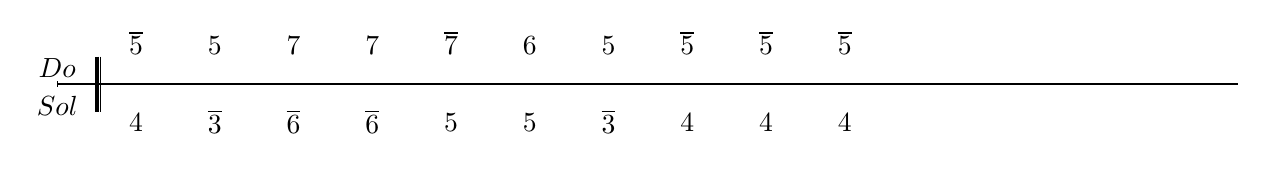
\begin{tikzpicture}
\newarray\North
\readarray{North}{5&5&7&7&7&6&5&5&5&5&}
\newarray\South
\readarray{South}{4&3&6&6&5&5&3&4&4&4&}
\draw[thick] (0,0) -- (15,0) node[anchor=north west] {}; % main ligne
\draw (0cm, 1pt) -- (0cm, -1pt) node [anchor=south] {$Do$};  % init ligne Do
\draw (0cm, 1pt) -- (0cm, -1pt) node [anchor=north] {$Sol$};  % init ligne Sol
\draw [line width=0.5mm ] (0.5cm, 10pt) -- (0.5cm, -10pt) node {}; % thick vertical ligne
\draw (0.55cm, 10pt) -- (0.55cm, -10pt) node {}; % second start vertical ligne
\foreach \x in {2,3,4,7}
\node[below] at (\x,-0.5){$\smash{\overline{\South(\x)}}$};
\foreach \x in {1,5,6,8,9,10}
\node[below] at (\x,-0.25){$\South(\x)$};
\foreach \x in {1,5,8,9,10}
\node[above] at (\x,0.25){$\smash{\overline{\North(\x)}}$};
\foreach \x in {2,3,4,6,7}
\node[above] at (\x,0.25){$\North(\x)$};
\end{tikzpicture}
  \end{center}
\end{figure}
\end{document}
